%-----------------------------------------------------------------------------
%
%               Template for sigplanconf LaTeX Class
%
% Name:         sigplanconf-template.tex
%
% Purpose:      A template for sigplanconf.cls, which is a LaTeX 2e class
%               file for SIGPLAN conference proceedings.
%
% Guide:        Refer to "Author's Guide to the ACM SIGPLAN Class,"
%               sigplanconf-guide.pdf
%
% Author:       Paul C. Anagnostopoulos
%               Windfall Software
%               978 371-2316
%               paul@windfall.com
%
% Created:      15 February 2005
%
%-----------------------------------------------------------------------------


\documentclass[preprint]{sigplanconf}

% The following \documentclass options may be useful:

% preprint      Remove this option only once the paper is in final form.
% 10pt          To set in 10-point type instead of 9-point.
% 11pt          To set in 11-point type instead of 9-point.
% authoryear    To obtain author/year citation style instead of numeric.

\usepackage{listings,xspace}
\usepackage{amsmath}
\usepackage{fontspec}
\usepackage{xcolor}
\usepackage{url}
\usepackage{todonotes}
\usepackage{comment}

\lstdefinelanguage{Scala}%
{morekeywords={abstract,case,catch,char,class,%
    def,else,extends,final,%
    if,import,%
    match,module,new,null,object,override,package,private,protected,%
    public,return,super,this,throw,trait,try,type,val,var,with,implicit,%
    macro,sealed,%
  },%
  sensitive,%
  morecomment=[l]//,%
  morecomment=[s]{/*}{*/},%
  morestring=[b]",%
  morestring=[b]',%
  showstringspaces=false%
}[keywords,comments,strings]%

% \lstset{language=Scala,%
%   mathescape=true,%
%   columns=[c]fixed,%
%   basewidth={0.5em, 0.40em},%
%   basicstyle=\tt,%
%   xleftmargin=0.0cm
% }

% \lstset{tabsize=2,
% basicstyle=\ttfamily\fontsize{9pt}{1em}\selectfont,
% commentstyle=\itshape\rmfamily,
% numbers=left, numberstyle=\scriptsize\color{gray}\ttfamily, language=scala,moredelim=[il][\sffamily]{?},mathescape=false,showspaces=false,showstringspaces=false,xleftmargin=15pt,escapechar=@, morekeywords=[1]{let,fn,val},deletekeywords={for},classoffset=0,belowskip=\smallskipamount
% }

\lstset{tabsize=2,
basicstyle=\ttfamily\fontsize{9pt}{1em}\selectfont,
commentstyle=\color{gray}\itshape\ttfamily,
language=scala,moredelim=[il][\sffamily]{?},mathescape=false,showspaces=false,showstringspaces=false,xleftmargin=15pt,escapechar=@, morekeywords=[1]{let,fn,val},deletekeywords={for},classoffset=0,belowskip=\smallskipamount
}

% \newcommand{\todo}{{\bf \colorbox{red}{\color{white}TODO:}}}
\newcommand{\ie}{{\em i.e.,~}}
\newcommand{\eg}{{\em e.g.,~}}
\newcommand{\term}[1]{\mbox{\texttt{#1}}}
\newcommand{\itl}[1]{\mbox{\textit{#1}}}

% commas and semicolons
\newcommand{\comma}{,\,}
\newcommand{\commadots}{\comma \ldots \comma}
\newcommand{\semi}{;\mbox{;};}
\newcommand{\semidots}{\semi \ldots \semi}

% spacing
\newcommand{\gap}{\quad\quad}
\newcommand{\biggap}{\quad\quad\quad}
\newcommand{\nextline}{\\ \\}
\newcommand{\htabwidth}{0.5cm}
\newcommand{\tabwidth}{1cm}
\newcommand{\htab}{\hspace{\htabwidth}}
\newcommand{\tab}{\hspace{\tabwidth}}
\newcommand{\linesep}{\ \hrulefill \ \smallskip}

% figures
\newcommand{\figurebox}[1]
        {\fbox{\begin{minipage}{\textwidth} #1 \medskip\end{minipage}}}
\newcommand{\twofig}[3]
        {\begin{figure*}[t]#3\ \hrulefill\
        \caption{\label{#1}#2}\end{figure*}}
\newcommand{\boxfig}[3]
        {\begin{figure*}\figurebox{#3\caption{\label{#1}#2}}\end{figure*}}
\newcommand{\figref}[1]
        {Figure~\ref{#1}}

% arrays
\newcommand{\ba}{\begin{array}}
\newcommand{\ea}{\end{array}}
\newcommand{\bda}{\[\ba}
\newcommand{\eda}{\ea\]}
\newcommand{\ei}{\end{array}}
\newcommand{\bcases}{\left\{\begin{array}{ll}}
\newcommand{\ecases}{\end{array}\right.}


\newcommand{\selfassembly}{\texttt{self-assembly~}}
\newcommand{\Selfassembly}{\texttt{Self-assembly~}}
\newcommand{\sselfassembly}{\texttt{self-assembly}}

\begin{document}

\setmainfont[Mapping=tex-text]{Times New Roman}
\setmonofont[Scale=0.8,BoldFont={Consolas Bold}]{Consolas}

\special{papersize=8.5in,11in}
\setlength{\pdfpageheight}{\paperheight}
\setlength{\pdfpagewidth}{\paperwidth}

\conferenceinfo{GPCE'14}{September 14--15, 2014, V\"{a}ster\r{a}s, Sweden}
\copyrightyear{2014}
\copyrightdata{978-1-nnnn-nnnn-n/yy/mm}
\doi{nnnnnnn.nnnnnnn}

% Uncomment one of the following two, if you are not going for the
% traditional copyright transfer agreement.

%\exclusivelicense                % ACM gets exclusive license to publish,
                                  % you retain copyright

%\permissiontopublish             % ACM gets nonexclusive license to publish
                                  % (paid open-access papers,
                                  % short abstracts)

% \titlebanner{banner above paper title}        % These are ignored unless
% \preprintfooter{short description of paper}   % 'preprint' option specified.

% Materialization: Pluggable Type System Extensions
% Generative Self-Assembly: Language Extensions and Datatype Generic Programming
% Self-Assembling Type System Extensions
% Type System Extensions Through Generative Self-Assembly
% Generative Self-Assembly: Language Extensions and Datatype Generic Programming
% Macrotechnology: Lightweight Language Extension and Datatype Generic Programming via Generative Self-Assembly
% Macrotechnology: Language Extension and Datatype Generic Programming via Generative Self-Assembly
% Macrotechnology: Blending Language Extension and Datatype Generic Programming via  Generative Self-Assembly
% Generative Self-Assembly: Lightweight Language Extension and Datatype Generic Programming, All-in-One
% Blending Language Extension and Datatype Generic Programming via Generative Self-Assembly

\title{Lightweight Language Extension and Datatype Generic Programming, All-in-One}
% \subtitle{Subtitle Text, if any}

\authorinfo{Heather Miller}
           {EPFL}
           {heather.miller@epfl.ch}
\authorinfo{Philipp Haller}
           {Typesafe, Inc.}
           {philipp.haller@typesafe.com}
\authorinfo{Bruno C. d. S. Oliveira}
           {The University of Hong Kong}
           {bruno@cs.hku.hk}

\maketitle

\begin{abstract}
This is the text of the abstract.
\end{abstract}

% \category{CR-number}{subcategory}{third-level}

% % general terms are not compulsory anymore,
% % you may leave them out
% \terms
% term1, term2

% \keywords
% keyword1, keyword2

\section{Introduction}

In programming many different types of values often require similar
functionality. For example it is common to use methods (or
functions) that compare two values for equality or produce a pretty
printed string representation of the value. Because such functionality
is so pervasive it is desirable to have some programming language support
that helps defining functions working over a large class of types.

The solutions offered by existing programming languages are quite
varied. Even when considering a single language, various different
designs can co-exist.  For example, in Java, every object has a few
methods, including \lstinline{toString}, \lstinline{equals},
\lstinline{clone} or \lstinline{hashCode}.  These methods provide a
simple default implementation. However most of the times the
programmer is supposed to override the methods to ensure proper
functionality. Some other methods or functionality, such as
serialization, are also quite common, but Java does not impose it on
every type. Instead Java takes a different design where if a class
implements a \lstinline{Serializable} interface then instances of
that class are automatically serializable. This is
quite convenient because the programmer does not have to write any
code for doing serialization. Still there is other functionality
that also makes sense in a large class of types for which Java
provides no special support.

Another approach to providing similar functionality for a large class
of types is to use type classes~\cite{}. Type classes provide a
mechanism where a certain functionality can be captured in an
interface. When programmers need certain types of values to support a
given functionality, they can implement an \emph{instance} of a type
class. 

A notable feature of type classes is their support for
\emph{retroactive extensibility}~\cite{}.  Retroactive extensibility means
that the functionality can be implemented \emph{after} the type or
class has been defined. This is in contrast with conventional OO
programming, where all methods (such as \lstinline{toString} or 
\lstinline{equals}) should be implemented together with the
definition of the class. Retroactive extensibility means that type
classes offer a lot of flexibility and possibility for customizing
behaviour. As a result several authors have argued for the software
engineering benifits of using type classes~\cite{}.

Because of the flexibility and extensibility of type classes, the
Scala language has embraced them~\cite{}. Scala provides some language
features that help using type classes more effectively. Today, type
class inspired designs are used by various libraries~\cite{}.  Type
classes solve the problem of defining some functionality for a large
class of types elegantly.

However there is still space for improvement. Consider again the way
serialization is done in Java. The language direct built-in support
for serialization and the programmer does not need to write how to serialize code
for particular classes!  In contrast with type classes the programmer
would need to define the serialization code for each class himself.
One could imagine that the serialization approach would also make
sense for other types of operations such as \lstinline{equals} or
\lstinline{toString}.  It would be very convenient if the language would
provide automatically sensible implementations of these operations!

While directly built-in \emph{language extensions} such as the
serialization mechanism are very convinient, they are also quite
inflexible. There are two essential problems:

\begin{itemize}
\item {\bf Lack of Customization:} The algorithm to do serialization
  is built-in the language. Because of that programmers using the
  language cannot control or customize how serialization works. For
  example it is not possible to adapt the serialization mechanism to
  work with other formats (such as JSON or XML).

\item {\bf Lack of Generality:} The serialization mechanism only
  works for a specific functionality: serialization. However, as we
  have argued, similar language extensions would make sense for other types 
  of operations. 
\end{itemize}

In this paper we show a general mechanism, called \sselfassembly, for doing \emph{lightweight
  language extensions} (LLEs). This mechanism solves both problems and
provides the best of two worlds: it has the extensibility and
customization advantages of type classes; and it has the automatic
implementation advantages of Java's serialization mechanism.  The key
idea is to provide programmers with a generic mechanism for doing automatic
implementations of type classes. This mechanism allows programmers 
to define their own generic functionality, such as serialization,
pretty printing or equality.

\Selfassembly uses Scala's \emph{type-safe macro
  system}~\cite{} and it allows generating \emph{efficient} code.  It
is inspired by existing approaches to \emph{datatype-generic
  programming} (DGP)~\cite{ComparingGPHaskellRodriquez,
  ComparingGPHaskellHinze}. DGP is an advanced form of generic
programming~\cite{}, where generic functions can be defined by
inspecting the structure of types. A goal of DGP is static
\emph{type-safety}. That is, if we define a generic function, then it
should be possible to type-check the definition of the generic
function. Any type-errors should be reported at compile-time and in
terms of the generic function code (but not in terms of generated
code, for example).The use of Scala's type-safe macro
system in our approach allow us to preserve the type-safety goal of
DGP while, at the same time, supporting the definition of efficient
generic functions.  As we discuss in detail in Section~\ref{} defining
generic functions that combine type-safety and efficiency is quite
challenging with other approaches.

Another distinctive feature of \selfassembly is the support for OO
features when defining generic functions. The vast majority of DGP 
approaches have been developed for Haskell. Haskell is a purely
functional language, that has considerable differences to OO languages
like Scala or Java. In particular, Haskell has no \emph{subtyping} or a
notion similar to \emph{object identity}. As a result directly porting
DGP approaches developed for Haskell is limiting because these
approaches cannot deal with subtyping or object identity. However,
these features need to be accountted by generic functions for OO 
languages. \Selfassembly provides the necessary mechanism to allow 
the definition of generic functions with both subtyping and object identity.

Using \sselfassembly, we have ported a full-featured serialization
framework for Scala~\cite{} as a generic function (or LLE). The
framework is full-featured in that it handles all object-oriented
concerns, such as subtyping polymorphism, object identity, as well as,
advanced features of the type system. In contrast to the original
implementation, which was developed in an ad-hoc way, the new
implementation reuses all the generic infrastructure of
\selfassembly. As a result the code for the serialization framework is
significantly shorter. Furthermore we have implemented various other
generic functions such as ...

Finally we also show a different application of LLEs: \emph{generic
  properties}. In \selfassembly it is also possible to define some
types of static program analysis, which guarantee that a certain
property holds. In particular we have implemented an
\emph{immutability checker}. If a class is immutable, the immutability
checker will generate a type class instance for that class that
certifies that property. It then becomes possible to
define functions that work only on types that are certified to be
immutable.  The immutability checker is defined with just a few lines
of code similarly to a generic function.

In summary the contributions of this paper are:

\begin{itemize}

\item {\bf \sselfassembly:} A framework for LLEs based on 
  type classes \emph{and} type-safe macros, which provides both
  \emph{efficiency} and \emph{type-safety}. The framework includes 
  several auxiliary definitions, such as generic queries and
  transformations, that help defining new LLEs.

\item {\bf a full-featured DGP approach for OOP:} \selfassembly 
  supports the definition of datatype-generic functions.
  Moreover the generic functions can deal with features present in
  production OO languages, including subtyping, object identity, 
  object graphs, and generics. 

\item {\bf support for generic properties:} \selfassembly also
  supports the definition of lightweight forms of static program analysis.
  We have implemented an immutability checker in \sselfassembly. 

\item {\bf a case study using serialization:} We evaluated the
  expressive power of \selfassembly by porting a full-featured
  serialization framework.

%the pattern isn't only good for standard DGP (that also happens
%  to be statically inlined and is faster than other DGP approaches),
% but since it's based on type classes generated at compile-time, it's
% possible to extend the language and compiler in a number of (local
% but) powerful ways (for example, transitive immutability checking)
% using this generative pattern.


%\item to reduce the amount of boilerplate for those wanting to use
% this generative pattern, we also provide a library for
%  query/transformation-based generic programming that can also be used
%  for these lightweight language.

\end{itemize}

% Programming often requires the definition of similar methods (or
% functions) for different types of values. Some of these methods are so
% common that certain languages simply assume that every value supports
% them.

% %% even if sometimes, for particular objects, the method in
% %%question does not make sense

% Very often the definition of such methods follows a common
% pattern. and some languages provide default implementations...

% Section 1:
%    - Programming requires many similar methods: toString, clone,
%       serialization ...
%    - A language can help by proving an implementation mechanism
%      (example serialization in Java), but this can be inflexible:
%      sometimes cannot override behaviour; cannot define an alternative
%      generic behaviour.
%    - DGP aims at allowing a flexible mechanism to do user-defined
%    generic functions;
%    - DGP explored extensibly in Haskell and Purely Functional
%    Programming.
%    - Much less work on OO languages. OO languages have challenges
%     that do not exist in pure languages like Haskell: Subtyping,
%     object graphs, general mutability
%    - How to do generic programming in OO languages
%    - Our solution using Scala macros to generate type class instances
%    - Making DGP efficient with macros (generating instances at compile
%    time). Treating type classes as first class entities
%    (double-check)?
%    - Case study: industrial strength serialization framework

% Section 2: Type Classes and the Boilerplate Problem
%   - What are type classes? (also introduce implicits)
%   - Show type class
%   - 3 instances: Int, List and Tree
%   - note that there is a similar pattern going on.

% Section 3: Basic selfassembly
%   - Show how to use the library to generate the instances and solve
%   the problem in Section 2; (What does the user have todo with your library?)
%   - Show how to define the ``generic function'' (What if a user wants to
%   define his own generic function?)
%   - explain the mechanisms involved (example, macros)
%   - Query Pattern? (here or somewhere else)?

% Section 4: Selfassembly for OO features
%   - Explain problem of object identity
%   - Subtyping
%   - Mutability? (Is this an issue?)

% Section 5: Language extensions with the selfassembly Library
%   - Show some more general patterns

% ...

% Section (n-1): Implementation and Case studies
%   - Tell about the implementation
%   - Tell about what generic functions have been implemented
%      and plans for more functionality

% Section n: Related work
%    - DGP in Haskell
%    - DGP in OO languages
%    - Compile-time reflection

% Question: What's meant by language extensions?
% quesries \& transformations (in the sense of SyB?)

% Question: How about producer generic functions? Example deserialize?

% Question: ``can use these generative techniques to extend the compiler and type system in local but powerful ways.''?


% full of d\'ej\`a vu moments. When a programmer writtes
% a new program, it is very likely that some similar pattern or
% functionality that

\begin{comment}
The text of the paper begins here.~\cite{ComparingGPHaskellRodriquez, ComparingGPHaskellHinze, ScalaGenericProgrammers, RepLib, OOGP}

Implicits are a huge deal, because they provide \textbf{extensibility.} Users can easily customize generated code by making use of implicits in Scala.


Contributions.

Implicits and macros powerful tools for doing generative programming. In fact, so powerful, that we can do more than inlined and performant datatype generic programming. We can use these generative techniques to extend the compiler and type system in local but powerful ways.

\begin{itemize}
\item library
\item pattern
\end{itemize}

We first describe what we call the ``self-assembly pattern'' -- a
technique for combining implicits and macros to generate complex in
Section~\ref{sec:self-assembly-pattern} to generate type class
instances.
\end{comment}

\section{Type Classes and a Boilerplate Problem}
% \label{sec:type-classes-and-boilerplate-problem}
\label{sec:background}

This section provides an introduction to type classes~\cite{} and
reviews how to encode them in Scala using implicits and conventional
OO features~\cite{Oliveira2010}.  This section also observes that type
classes instances for various types tend to require code that follows
a common pattern. The pattern can be viewed as a source of code
boilerplate, since similar code needs to be repeated throughout several
definitions. The remainder of the paper aims at showing how
to capture the pattern as reusable code and generate type class
instances automatically from that code.


%\subsection{Singletons}
% \label{sec:singletons}
%
% ...
%
% \paragraph{Companion Objects} ...
% \end{comment}

\subsection{Implicits}
\label{sec:implicits}

In Scala, it is possible to select values
automatically based on type. These capabilities are enabled when using the
\term{implicit} keyword. For example, a method \term{log} with multiple
parameter lists may annotate their last parameter list using the
\term{implicit} keyword.%%\footnote{Example taken from~\cite{Oliveira2010}.}

\begin{lstlisting}
def log(msg: String)(implicit o: PrintStream) =
  o.println(msg)
\end{lstlisting}

This means that in an invocation of \term{log}, the implicit argument list may
be omitted if, for each parameter of that list, there is exactly one value of
the right type in the {\em implicit scope}. The implicit scope is an
adaptation of the regular variable scope; imported implicits, or implicits
declared in an enclosing scope are contained in the implicit scope of a method
invocation.

\begin{lstlisting}
    implicit val out = System.out
    log("Does not compute!")
\end{lstlisting}

In the above example, the implicit val \term{out} is in the implicit scope of
the invocation of \term{log}; since it has the right type, it is automatically
selected as an implicit argument.

%\todo Maybe we should change this example? It's out of Bruno's paper, and he's
%on the committee, he'll probably review our paper.

%\todo Talk about how we use implicit values in our framework here.

\begin{comment}
\paragraph{Implicit Conversions.} Implicit conversions can be thought of as
methods which, like implicit parameters, can be implicitly selected (\ie
invoked) based upon their type, and whether or not they are present in
implicit scope. As with implicit parameters, implicit conversions also carry
the \term{implicit} keyword before their declaration.

\begin{lstlisting}
 implicit def intWrapper(x: Int): Message =
    new Message {
      def message: String = "secret message!"
    }
\end{lstlisting}

In the example above, assuming there exists an abstract class \term{Message}
with abstract method \term{message}, the implicit conversion
\term{intWrapper} will be triggered when a method called \term{message}
is called on an \term{Int}. That is, simply calling
\term{39.message} will result in ``secret message!'' being
returned. Since the implicit conversion has the effect of adding a
``new'' method to type \term{Int}, \term{message} is typically called an
{\em extension method}. In our framework we use implicit conversions,
for example, for adding a \term{pickle} method to arbitrary objects.
\end{comment}

% cite Adriaan's and Bruno's OOPSLA paper. Where? How?
% Example of a type class: maybe Ordering type class of std lib?
% Include info on importing implicit values, and implicit resolution by scoping.
% Example of a plain implicit parameter: could use implicit ExecutionContext in futures

% \subsection{Reflection}
% \label{sec:reflection}

% Reflection is the ability of a program to inspect, and possibly even modify
% itself at runtime. Before Scala 2.10, Scala did not have any reflection
% capabilities of its own. Instead, one could use Java reflection which provided
% basic but limited runtime reflection capabilities. In Scala 2.10, a new
% reflection library was introduced not only to address the shortcomings of
% Java's runtime reflection on Scala-specific and generic types, but to also add
% a more powerful toolbox of general reflective capabilities to Scala. Along
% with full-featured runtime reflection for Scala types and generics, Scala 2.10
% also ships with compile-time reflection capabilities, in the form of macros
% (covered in Section \ref{sec:macros}), as well as the ability to reify Scala
% expressions into abstract syntax trees.

% \paragraph{TypeTags.} One aspect of runtime reflection that was introduced in
% Scala 2.10 is the notion of \verb|TypeTag|s. As with other JVM languages,
% Scala's types are erased at compile time. \verb|TypeTag|s can be thought of as
% objects which carry along all type information available at compile time, to
% runtime. As we will see, \verb|TypeTag|s will prove to be invaluable in
% situations where precise type information would otherwise not be available at runtime.

% \paragraph{Unified Runtime/Compile-time Reflection API.} Another important
% aspect of Scala's reflection library is the one-to-one correspondence between
% Scala Reflection's compile-time (\ie macros) and runtime APIs. Each API is
% parameterized on a so-called \verb|Universe|, an object which serves as the
% entry point to Scala reflection, and which provides all principal concepts
% used in reflection, such as \verb|Type|s, \verb|Tree|s, and
% \verb|Annotation|s. Depending on the task at hand, the choice between runtime
% and compile-time reflection is as easy as selecting either a compile-time or a
% runtime \verb|Universe|. As we will see, this enables maximum code
% reuse in that a fallback runtime pickler generation mechanism can be achieved
% by simply reusing the code for static generation, and parameterizing it on a
% runtime \verb|Universe|.

\subsection{Type Classes}
\label{sec:type-classes}

Type classes are a language mechanism that provide a disciplined
alternative to ad-hoc polymorphism. They have been popularized by
Haskell, but several other languages have adopted similar ideas.  Type
classes allow functions to be defined over a set of types.  If values
of a type \lstinline{T} should provide a certain functionality then that
functionality can be specified as an \emph{instance} of a type class.

\begin{figure}
\begin{lstlisting}
// Show type class
trait Show[T] {
  def show(visitee : T) : String
}

// Show instance for integers
implicit object IntInstance extends Show[Int] {
  def show(o : Int) = o.toString()
}
\end{lstlisting}
\caption{\lstinline{Show} type class and corresponding instance for
  integers.}
\label{fig:showtc}
\end{figure}

In Scala type classes can be implemented using a combination of
standard OO features (traits, classes and objects) and implicits.
The Scala encoding of type classes is essentially a \emph{design pattern}~\cite{}:
instead of having built-in language concepts for type classes, Scala
uses general language features to model type classes.
A type class is simply an interface that provides operations
over one (or more) generic types. Such interfaces can be modeled
as traits in Scala. An example of a type class is shown in
Figure~\ref{fig:showtc}. The trait \lstinline{Show[T]} models a type
class that provides pretty printing functionality for some type
\lstinline{T} via a method \lstinline{show}.

The main conceptual difference between standard OO methods and
type-class methods is that the later are provided \emph{externally} to
objects. For example suppose that we wanted to add pretty printing
functionality to integers. To do this we could create an instance of
the type class Show where the generic type parameter \lstinline{T} is
instantiated to \lstinline{Int}. The \lstinline{object IntInstance} in
Figure~\ref{fig:showtc} illustrates how to model such instance in
Scala using regular objects. In that object, the \lstinline{show}
method takes an argument \lstinline{o} of type \lstinline{Int} an
invokes the \lstinline{toString()} method on \lstinline{o}.
%%To use the pretty printing functionality in client code we could create
%%a method \lstinline{eshow}:

%%begin{lstlisting}
%%// explicitly taking instance argument
%%def eshow[T](o : T)(showT : Show[T]) = showT.show(o)
%%\end{lstlisting}

%%This method takes an object \lstinline{o} of some generic type \lstinline{T} and
%%an instance \lstinline{showT} of type \lstinline{Show[T]} and applies
%%the \lstinline{show} method in \lstinline{showT} to \lstinline{o}.
%%With \lstinline{eshow} we could

\paragraph{Type-Directed Resolution of Instances} An interesting
aspect of type classes is that instances can be automatically
determined using a type-directed resolution mechanism. This
type-directed resolution mechanism allows type classes
to be used from client code through a mechanism similar to
overloading. One way to achieve this is Scala is using an implicit
parameter:

\begin{lstlisting}
// show with implicit parameter
def ishow[T](v : T)(implicit showT : Show[T]) =
  showT.show(v)
\end{lstlisting}

In \lstinline{ishow} the idea is that the method takes two parameters,
with the last of these (\lstinline{showT}) being implicit. As we have
seen in Section~\ref{sec:implicits} this means that the second
parameters can be automatically determined by the compiler.  For
example if we wanted to use \lstinline{show} on integers we could
simply write a program such as:

\begin{lstlisting}
def test1 = ishow(5)
\end{lstlisting}

Provided that an \lstinline{implicit} value of type
\lstinline{Show[Int]} is in the implicit scope (for example
\lstinline{IntInstance} from Figure~\ref{fig:showtc}), the second
parameter is automatically inferred by the compiler.

\paragraph{Context Bounds} Type classes are pervasivaly used in
Scala. Because of this Scala offers an alternative convinient syntax sugar called
\emph{context bounds}. Context bounds allows code using type classes to be
written more compactly and arguably more intuitively. With context
bounds, instead of writting \lstinline{ishow} we could write:

\begin{lstlisting}
// show with context bounds
def show[T : Show](v : T) =
  implicitly[Show[T]].show(v)
\end{lstlisting}

The idea of context bounds comes from the fact that type classes can
also be seen as a generic programming mechanism~\cite{}, which allows
generic parameters to be constrained. In this case the type of
\lstinline{show} can be read as a generic method where the generic
type argument must be an instance of \lstinline{Show}.
A small problem with context bounds there is no parameter name to be used in the
definition of \lstinline{show}. However, it is possible to
\emph{query} the implicit scope for a value of a certain type
using a simple auxiliary method called \lstinline{implicitly}:

\begin{lstlisting}
def implicitly[T](implicit x : T) : T = x
\end{lstlisting}

This precludes the need for having to have the name of the implicit
argument in hand in order to use it.
From the client perspective, using \lstinline{show} is similar to
using \lstinline{ishow}.

\subsection{Pretty Printing Complex Structures}\label{sec:pretty-printing-complex}

\begin{figure}
\begin{lstlisting}
sealed trait Tree
case class Fork(left : Tree, right : Tree)
  extends Tree
case class Leaf(elem : Int) extends Tree

implicit object TreeInst extends Show[Tree] {
 def show(visitee : Tree) : String =
   visitee match {
     case Fork(l,r) =>
       "Fork(" + show(l) + ", " + show(r) + ")"
     case Leaf(x) => "Leaf(" + x.toString() + ")"
   }
}
\end{lstlisting}
\caption{Trees of integers and corresponding \lstinline{Show}
  instance.}
\label{fig:trees}
\end{figure}

Of course it is also possible to apply type classes to more complex
structures. For example consider a simple type of binary trees with
integers at the leafs. Figure~\ref{fig:trees} shows how to model such
trees in Scala using \emph{case classes}~\cite{} and \emph{sealed
  traits}. The keyword \lstinline{sealed} in Scala means that the
trait can only be implemented by definitions in the existing module.
Any definition outside the module will not be able to implement the
trait. Together with case classes this allows modeling \emph{algebraic
  datatypes}, which are a well-know concept from functional programming.
The \lstinline{Tree} trait is the type of trees. The case class
\lstinline{Fork} models the binary nodes of the tree, wheres the case
class \lstinline{Leaf} models the leafs containing an integer value.

To define pretty printing for \lstinline{Tree} using the
\lstinline{Show} type class we create an \lstinline{object TreeInst}.
This object provides a definition for the
\lstinline{show} method that pattern matches on the
two tree constructors (cases) of \lstinline{Tree}. The implementation
of the two cases is unremarcable: in both cases the
constructors names and the arguments are printed.

A simple test program illustrating the use of \lstinline{TreeInst}
is shown next:

\begin{lstlisting}
val tree : Tree = Fork(Fork(Leaf(3),Leaf(4)),Leaf(5))
def test3 = show(tree)
\end{lstlisting}

\noindent The value \lstinline{tree} defines a simple tree and the
definition \lstinline{test3} pretty prints that tree.

\begin{figure}
\begin{lstlisting}
sealed trait PTree[A]
case class Branch[A](x : A, l : PTree[A], r : PTree[A])
  extends PTree[A]
case class Empty[A] extends PTree[A]

implicit def PTreeInst[A : Show] : Show[PTree[A]] =
  new Show[PTree[A]] {
    def show(visitee : PTree[A]) =
     visitee match {
        case Branch(x,l,r) =>
           "Branch(" + implicitly[Show[A]].show(x) +
           ", " + show(l) + ", " + show(r) + ")"
   	    case Empty() => "Empty()"
     }
}
\end{lstlisting}
\caption{Parametrized trees and corresponding \lstinline{Show}
  instance.}
\label{fig:ptrees}
\end{figure}

\paragraph{Recursive Resolution and Compositionality of Instances}
Another interesting aspect of type classes is that they provide a
highly compositional way to define instances for parametrized types.
Lets consider a variant of trees, shown in Figure~\ref{fig:ptrees}, which is
parametrized by some element type \lstinline{A}. The type these trees
is \lstinline{PTree[A]} and there are two types of nodes:
\lstinline{Branch} nodes with an element of type \lstinline{A}
and two branches; and \lstinline{Empty} nodes with no content.

Like other types it is possible to define an instance (\lstinline{PTreeInst})
for the type \lstinline{PTree[A]}. However in order to pretty pretty
such trees it is necessary to know how to print the elements of type
\lstinline{A} as well. To accomplish this we require that the
generic type parameter \lstinline{A} has a \lstinline{Show} instance
using a context bound.  To print the elements in the
\lstinline{Branch} case, the instance can be retrieved from the local
scope using \lstinline{implicitly} and then used to print the element.
With this instance it is possible to print trees with integer elements, such as:

\begin{lstlisting}
val ptree : PTree[Int] = Branch(5,Empty,Empty)
def test4 = show(ptree)
\end{lstlisting}

However, more interestingly, it is also possible to print trees where
for any element type that has a \lstinline{Show} instance. For example:

\begin{lstlisting}
val ptree2 : PTree[PTree[Tree]] =
  Branch(Branch(tree,Empty,Empty),Empty,Empty)
def test5 = show(ptree2)
\end{lstlisting}

Here \lstinline{ptree2} has element types of type
\lstinline{PTree[PTree[Tree]]}. To print the trees the instance for
\lstinline{PTree} has to be used twice: one to print values of type
\lstinline{PTree[PTree[Tree]]}; and another time to print values of
type \lstinline{PTree[Tree]}. In fact it is possible to use
arbitrarely many instances of the various types (possible multiple
times) during type-directed resolution, which makes the process very
compositional. This is possible because the type-directed resolution
mechanism is recursive.

\subsection{A Boilerplate Problem}

Although type classes are nice, they often require similar code for
different instances. For example consider the two instances
in Figures~\ref{fig:trees} and~\ref{fig:ptrees}. The code that is
needed in both instances is quite similar and it follows a common
pattern: for each case the constructor name and parameters are
printed. Therefore code tends to be quite similar across instances. This
code can be viewed as a form of boilerplate since we could hope that
it could be mechanically generated. However, at the moment the code
is being defined by hand for each instance.

%Both \lstinline{ishow} and \lstinline{show}
%provide a convenient way for some client code to invoke the pretty
%printing functionality on some values of type \lstinline{T}.

\begin{comment}
\begin{lstlisting}
// Adding a show method to an arbitrary
// object of a certain type
trait Showable {
 def show() : String
}

implicit def showWrapper[T : Show](visitee : T) =
 new Showable {
   def show() = implicitly[Show[T]].show(visitee)
 }

def test2 = 5.show()
\end{lstlisting}
\end{comment}






% \begin{comment}
\section{Type-Safe Meta-Programming in Scala}
\label{sec:macros}

Scala macros~\cite{Burmako2012, Burmako2013} enable a form of type-safe
meta-programming. Macros are methods that are invoked at compile time; instead of
runtime values, macros operate on and return typed expression trees. In the
following we provide an overview of macros, type checking, and usage
restrictions; in addition, we introduce quasiquotes as a high-level API
for working with expression trees.

\paragraph{Definition} Macro defs are methods that are transparently loaded by
the compiler and executed (or expanded) during compilation. A macro is defined
like any normal method, but it is linked using the \verb|macro| keyword to an
additional method that provides its implementation, which operates on
expression trees. Example:
\begin{lstlisting}
def assert(x: Boolean, msg: String): Unit =
  macro assert_impl
def assert_impl(c: Context)
  (x: c.Expr[Boolean], msg: c.Expr[String]):
                            c.Expr[Unit] = ...
\end{lstlisting}
\noindent
In the above example, the parameters of \verb|assert_impl| are typed
expression trees, which the body of \verb|assert_impl| operates on, itself
returning an expression of type \verb|Expr[Unit]|. It is \verb|assert_impl|
which is expanded and evaluated at compile time; its result is then inlined at
the call site of \verb|assert| and the inlined result is type-checked.

Note that expression trees are typed, \ie \verb|assert|'s parameter of type
\verb|Boolean| corresponds to a typed expression tree of type
\verb|Expr[Boolean]|. There are two choices available for building expression
trees: (a) via \verb|reify| and (b) via quasiquotes (see below):
\begin{lstlisting}
val expr: c.Expr[Boolean] = reify {
  if (x.splice > 10) x.splice
  else true
}
\end{lstlisting}
\noindent
Here, the body of \verb|reify| consists of regular Scala code; expressions in
the enclosing scope are spliced into the result expression using the
\verb|splice| method. Importantly, the code within \verb|reify| is
type-checked at its definition site. This means, for the above code, Scala's type
checker reports a type error, not in terms of the generated code, but in terms
of the high-level typed expression trees.

An alternative to working with \verb|reify|/\verb|splice| are quasiquotes.
Quasiquotes are an experimental feature of Scala 2.11 which simplify working
with expression trees. They allow splicing trees similar to Scala's standard
string interpolation:
\begin{lstlisting}
def assert_impl(c: Context)
  (x: c.Expr[Boolean], msg: c.Expr[String]):
                            c.Expr[Unit] =
  c.Expr[Unit](q"if (!$x) error($msg)")
\end{lstlisting}
\noindent
Currently, quasiquotes are type-checked during macro expansion, but are
planned to soon be type-checked prior to expansion.



% - full description of macros
% - how are things type-checked: when, what happens when there are errors
% - footnote: whitebox macros are another form of macros which ...
% - interactions, important details

% don't have access to mutate symbol table
% - for these reasons they're much more principled than approaches like TH.

% - quasi-quotes, splicing trees




% It is also important to note that implicit defs as described earlier
% in Section \ref{sec:implicits} can be implemented as macros.

As we will see, these macros defs, coupled with implicits in Scala enable the
boilerplate-free type class instance synthesis.
% Scala pickling framework at the pickling use-
% site.

% \paragraph{Macro Annotations.} Unlike macro defs, macro annotations are capable
% of {\em adding members} to classes which carry their annotation.

% \begin{lstlisting}
% @withNewToString
% class D { ... }
% \end{lstlisting}

% The \verb|withNewToString| annotation is defined using a standard class
% definition by extending a special \verb|MacroAnnotation| marker trait, and by
% implementing a special \verb|transform| method as a macro:

% \begin{lstlisting}
% class withNewToString extends MacroAnnotation {
%   def transform = macro transform_impl
%   def transform_impl = { ... }
% }
% \end{lstlisting}

% The \verb|transform| macro implementation is passed the AST of the annotated class
% definition (the AST of ``\verb|class D { ... }|''), and returns a possibly changed AST
% as the new class definition (which could have added members, changed
% constructor parameters etc.)
% \end{comment}

% Section 2:
% explain how to write type classes manually

\section{Basic Self-Assembly}
\label{sec:basic-self-assembly}

% This is how we can write type classes using the selfassembly library
% This is quite short!
% After that we explain how it's actually generated!
% It's a pattern that generalizes the way one typically writes type classes by hand.

The previous section showed how to write type classes like \verb|Show[T]|
manually, pointing out a source of significant boilerplate code. In
section~\cite{sec:basic-usage}, we outline the basic usage of the
\selfassembly library, which allows defining type classes desired in a way
where the required boilerplate is generated for you.
Section~\ref{sec:basic-generation} explains the mechanics of the automatic
type class generation implemented in the \selfassembly library.
Section~\cite{sec:customization} outlines how one can customize the generation
of type classes for specific types.

\subsection{Basic Usage}
\label{sec:basic-usage}

\begin{figure}
\centering
\begin{lstlisting}
object Show extends Query[String] {
  def mkTrees[C <: SContext](c: C) = new Trees(c)

  class Trees[C <: SContext](override val c: C)
      extends super.Trees(c) {
    import c.universe._
    type SExpr = c.Expr[String]

    def combine(left: SExpr, right: SExpr) =
      c.Expr(q"$left + $right")

    def delimit(tpe: c.Type) = {
      val start = tpe.typeSymbol.name.toString + "("
      (c.Expr(q"$start"), reify(", "), reify(")"))
    }
  }

  implicit def generate[T]: Show[T] =
    macro genQuery[T, this.type]
}
\end{lstlisting}
  \caption{Implementing a type class using \selfassembly}
  \label{fig:basic-usage}
\end{figure}

The \selfassembly library allows implementing type classes in a way such that
instances for a large class of types are generated automatically, on-the-fly.
This section introduces the library using the simple \verb|Show| type class
introduced in Section~\ref{sec:type-classes}. Section~\ref{sec:queries-transformations}
shows how our approach extends to different forms of type classes, commonly referred to
as queries and transformations (TODO: cite papers).

\paragraph{Generating Instances for \texttt{Show}} Suppose a user would like
to provide instances of \verb|Show[T]| for as many
types as possible. Using \selfassembly it's sufficient to create a singleton
object that extends a library-provided trait, and that implements two factory
methods, \verb|generate| and \verb|mkTrees|, as follows.
Figure~\ref{fig:basic-usage} shows the \verb|Show| companion object,\footnote{A companion
object is a singleton object with the same name as a trait...} which extends
the \verb|Query| trait. The \verb|mkTrees| factory method, abstract in \verb|Query|,
creates a new \verb|Trees| instance; \verb|Trees[C]| provides a number of methods that
are invoked by the \selfassembly library at \emph{compile time} to obtain AST fragments that are
inlined in the generated code. The \verb|Show| type class converts objects to
strings; thus, the query has to define how to assemble result strings, based
on an associative combination operator (\verb|combine|), begin/end delimiters
(\verb|first|/\verb|last|), and a separator. The syntax
\verb|q"$left + $right"| denotes a \emph{quasiquote}~\cite{Quasiquotes},
creating an AST node using Scala code, where \verb|left| and \verb|right|
are tree nodes that are spliced into the result node.

Apart from implementing a subclass of \verb|Trees[C]|, the \verb|Show|
singleton object also needs to define a generic implicit method (here,
\verb|generate|) that invokes the generation macro \verb|genQuery|. The
\verb|genQuery| macro is provided by our library.\footnote{The type argument
\texttt{this.type} is the type of the enclosing singleton object; it is passed
to \texttt{genQuery} to identify the type class and the \texttt{mkTrees}
method that should be used by the library to generate instances.}

\paragraph{Result} With the \verb|Show| singleton object defined as in Figure~\ref{fig:basic-usage}
it is no longer necessary for the user to define a type class instance for every single type manually.
Instead, whenever an instance of type, say, \verb|Show[MyClass]|, is required
(typically, using an implicit parameter), Scala's type checker automatically inserts
a call to the \emph{implicit def} \verb|generate[MyClass]|; this implicit def generates a
suitable implementation of the searched type class instance on-the-fly. As a result,
type class instances do not have to be defined manually.

\subsection{Generation Mechanism}\label{sec:basic-generation}

% high-level overview of the pattern. macros generate calls to
% \\\verb|implicitly[T]| and generate the bodies of implicit objects. the
% macro also inspects the type and based on that, generates nested
% \verb|implicitly[S]| calls. these calls are resolved either using regular
% implicits, or by expanding the implicit macro recursively.

% We start with a simplified view of types in Scala. In subsequent sections we
% show how to generalize this view to richer types.

\begin{figure}
  \centering
$\ba[t]{l@{\hspace{2mm}}l@{\hspace{2mm}}}
T    ::= & \texttt{sealed trait}~C~\{~\bar{m}~\} \\
\gap ~|~ & \texttt{case class}~C(v~p_1: D_1, \ldots, v~p_n: D_n)~\{~\bar{m}~\} \\
\gap     & \texttt{~~extends}~E_1~\texttt{with}~ \ldots ~\texttt{with}~E_m \\
v    ::= & \texttt{var} \\
\gap ~|~ & \epsilon \\
m    ::= & \ldots \\
\ea$
  \caption{Grammar for simple datatypes in Scala.}
  \label{fig:type-syntax}
\end{figure}

We begin by illustrating the general idea of our generation technique through
a simple example that is itself based solely on closed ADT-style datatypes in
Scala, which can be described using the grammar in
Figure~\ref{fig:type-syntax}.\footnote{Case classes are considered to be
final, even though in the current version of Scala they can technically be
extended; extension is deprecated, though.} In subsequent sections we show how
to generalize this view to richer types.

Our treatment is centered on an example, in which, our goal is to
automatically ``derive'' type class instances that ``show'' information about
a given type. Think of it as a \verb|toString| method that traverses the
structure of a type, and nicely prints information about all of the fields of
that type.

We structure our treatment into three distinct steps (described in the
corresponding subsections):

\begin{enumerate}
\item In Section~\ref{sec:triggering-generation}, we show how our generation is
      triggered.

\item In Section~\ref{sec:macro-based-generation}, we explain our macro-based
      generation technique.

\item In Section~\ref{sec:generated-type-class-instances}, we show some example
      type class instances that result from our generation technique, and relate
      them to the type class pattern introduced in Section~\ref{sec:type-classes}
\end{enumerate}

\subsubsection{Triggering generation}
\label{sec:triggering-generation}

To be able to generate suitable instances for all possible types for which
\verb|Show[T]| can be defined, we put an implicit macro into the companion
object of \verb|Show[T]|. The fact that the implicit macro is inside the
companion object means that whenever an instance \verb|Show[S]| is requested,
Scala's implicit lookup mechanism searches the members of the companion object
\verb|Show| where it finds the implicit macro:

\begin{lstlisting}
object Show extends Query[String] {
  ...
  implicit def generate[T]: Show[T] =
    macro genQuery[T, this.type]
}
\end{lstlisting}
\noindent
Thus, the implicit lookup mechanism inserts an invocation of the macro method
\verb|genQuery|.

\subsubsection{Macro-based generation}
\label{sec:macro-based-generation}

Being a macro, \verb|genQuery| returns an abstract syntax
tree instead of a (runtime) value. It is declared as follows:

\begin{lstlisting}
def genQuery[T:c.WeakTypeTag, S:c.WeakTypeTag]
    (c: Context): c.Tree = ...
\end{lstlisting}
\noindent
Note that in this declaration, the type parameters \verb|T| and \verb|S| are annotated with
so-called \emph{context bounds} \verb|c.WeakTypeTag|. Context bounds are an
alternative way of adding synthetic implicit parameters:

\begin{lstlisting}
def genQuery[T, S](c: Context)
  (implicit ev1: c.WeakTypeTag[T],
            ev2: c.WeakTypeTag[S]): c.Tree = ...
\end{lstlisting}
\noindent
The evidence parameters \verb|ev1| and \verb|ev2| of type \verb|c.WeakTypeTag[T]| provide
access to the full static type information of types \verb|T| and \verb|S|.

% The \verb|genQuery| macro inspects this type information to generate a value of
% the following shape:

% \begin{lstlisting}
% implicit object $instanceName extends Show[T] {
%   def show(visitee: T): String = $tree
% }
% $instanceName
% \end{lstlisting}
% \noindent
% As required, the generated value has type \verb|Show[T]|. Hygiene requires the
% macro to generate a fresh (term) name \verb|$instanceName|. The actual
% implementation of the type class (\verb|$tree|) is generated as follows.

First, the macro collects essential information about the types and the type
class for which an instance should be generated. Second, the macro creates an
instance of the user-provided \verb|Trees| class by invoking the
\verb|mkTrees| factory method. These steps are shown in Figure~\ref{fig:macro-set-up}.

\begin{figure}
\centering
\begin{lstlisting}
trait Query[R] ... {

  def mkTrees[C <: Context with Singleton](c: C)
    : Trees[C]

  abstract class Trees[C <: Context with Singleton]
    (override val c: C) extends super.Trees(c) { }

  def genQuery[T:c.WeakTypeTag, S:c.WeakTypeTag]
    (c: Context): c.Tree = {
    import c.universe._

    val tpe = weakTypeOf[T]
    val stpe = weakTypeOf[S]
    val tpeOfTypeClass =
      stpe.typeSymbol.asClass.companion.asType
          .asClass.toTypeConstructor
    val qresTpe =
      tpeOfTypeClass.decls.head.asMethod.returnType

    val trees = mkTrees[c.type](c)
    ...
\end{lstlisting}
  \caption{Macro-based generation: set-up}
  \label{fig:macro-set-up}
\end{figure}

The body of the type class is generated using the following
quasiquote:\footnote{For simplicity and not to obscure the presentation we are
not concerned about hygiene.}

\begin{lstlisting}
val acc = c.Expr[R](q"combineResult")
val postfixTree = c.Expr[R](q"postfix")
q"""
  var combineResult: $qresTpe = ${trees.first(tpe)}
  ..$fieldTrees // (list of trees)
  val postfix: $qresTpe = ${trees.last(tpe)}
  combineResult = ${trees.combine(acc, postfixTree)}
  combineResult
"""
\end{lstlisting}
\noindent

The quasiquote produces an AST which constitutes the implementation of the
single abstract method of the type class. The AST returns the value of
\verb|combineResult|, a local variable of type \verb|R|, the type parameter of
\verb|Query[R]| within which the macro is defined; \verb|R| is the return type
of the type class method (\eg \verb|String| in the case of \verb|Show|). The
value of \verb|combineResult| is the result of combining the following pieces:
first, the initial result returned by the AST \verb|trees.first(tpe)|; second,
the results returned by nested invocations of the type class on fields;
finally, the result returned by the AST \verb|trees.last(tpe)|. To obtain
those ASTs, the macro utilizes the \verb|trees| instance (of type
\verb|Trees|) that was constructed in the set-up phase (see Figure~\ref{fig
:macro-set-up}). Moreover, all these fragments are combined using the AST
returned by \verb|trees.combine(acc, postfixTree)|.

The list of ASTs \verb|fieldTrees| is obtained as follows. For each field
declared in type \verb|tpe|, the following subtree is generated:

\begin{figure}
\centering
\begin{lstlisting}
val symTp = sym.typeSignatureIn(tpe)
val fieldName = sym.name.toString.trim
val valueTree = trees.fieldValueTree(fieldName,
                  symTp, tpeOfTypeClass)
val next = c.Expr[R](q"res")
val sepTree =
  if (isFirst) { isFirst = false; q"" }
  else q"combineResult =
    ${trees.combine(acc,
                    trees.separator).tree}"
q"""
  $sepTree
  val res: $qresTpe = $valueTree
  combineResult = ${trees.combine(acc, next).tree}
"""
\end{lstlisting}
  \caption{desc.}
  \label{fig:macro-combine-result}
\end{figure}

Of all these subtrees,
\verb|trees.fieldValueTree(fieldName, symTp, tpeOfTypeClass)| is most interesting.
It expands to a nested look-up of a type class instance for the field, as well as
an invocation of the type class method. Figure~\ref{fig:macro-field-value} shows its implementation.
The AST returned by \verb|implicitlyTree(tpe, tpeOfTypeClass)| is expanded as follows,
obtaining a type class instance for the current field:
\begin{lstlisting}
val instType = appliedType(tpeOfTypeClass, tpe)
q"implicitly[$instType]"
\end{lstlisting}


\begin{figure}
\centering
\begin{lstlisting}
def fieldValueTree(name: String, tpe: c.Type,
                   tpeOfTypeClass: c.Type): c.Tree = {
  val instTree   = q"inst"
  val fieldTree  = q"value"
  val invokeTree = invoke(instTree, fieldTree)
  q"""
    val inst = ${implicitlyTree(tpe, tpeOfTypeClass)}
    val value = visitee.${TermName(name)}
    $invokeTree
  """
}
\end{lstlisting}
  \caption{Nested implicit look-ups of instances}
  \label{fig:macro-field-value}
\end{figure}



% All methods are the \verb|Trees| class are provided by the library, although some of these methods are abstract

\subsubsection{Generated Type Class Instances}
\label{sec:generated-type-class-instances}

The generation technique explained in the previous section produces implicit
(singleton) objects which correspond to the type class intances portion of the
type class pattern introduced in Section~\ref{sec:type-classes}.

Let's say the datatype that we'd like to call \verb|show| on is a closed
ADT for binary trees, which looks like:

\begin{lstlisting}
sealed trait Tree
case class Fork(left: Tree, right: Tree)
  extends Tree
case class Leaf(elem: Int) extends Tree
\end{lstlisting}
\noindent

As one might infer, in order to create type class instances of type
\verb|Show[Tree]|, one must be able to create type class instances for
\verb|Tree|'s two subclasses, \verb|Fork|, and \verb|Leaf|. Since both
\verb|Fork| and \verb|Leaf|.

Note that \verb|Fork| and \verb|Leaf| are each case classes with the general
shape:

\begin{math}
\texttt{case class}~C(p_1: D_1, \ldots, p_n: D_n)~\{~\bar{m}~\} \\
\texttt{~~~~~extends}~E_1~\texttt{with}~ \ldots ~\texttt{with}~E_m
\end{math}
\noindent

An arbitrary type class instance (implicit singleton object) can be generated
using the technique described in the previous section which corresponds to the
arbitrary shape of $C$:

\begin{figure}[h!]
\centering
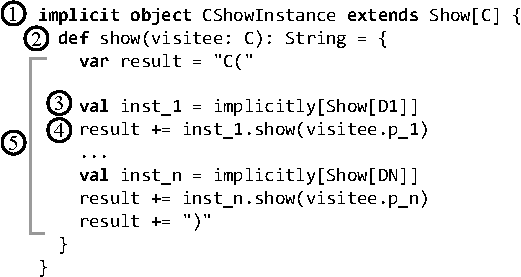
\includegraphics[width=0.87\columnwidth]{basic-generation.pdf}
\caption{desc.}
\label{fig:basic-generation}
\end{figure}

As we can see, the implicit object (1) in Figure~\ref{fig:basic-generation} is
exactly the same as in the manual type class pattern described in
Section~\ref{sec:type-classes}. (2) is the the implementation of the single
abstract method of the type class (the \verb|show| method of the \verb|Show|
trait). (3) is the result of expanding the \verb|implicitlyTree| invocation
shown in Figure~\ref{fig:macro-field-value}. (4) corresponds to the
accumulation logic which itself results from the expansion of
\verb|combineResult| shown in Figure~\ref{fig:macro-combine-result}. Finally,
(5) corresponds to the expansion of \verb|trees.first| and \verb|trees.last|
in the body of the macro-generated implementation of \verb|Show|'s single
abstract method, \verb|show|.



% To understand the self-assembly pattern, we use the following example.
% Given an ADT for binary trees storing \verb|Int|s modeled as follows:

% In this example, our goal is to automatically ``derive'' type class instances
% that ``show'' information about a given type. Think of it as a \verb|toString|
% method that traverses the structure of a type, and nicely prints information
% about all of the fields of that type.

% The \verb|Show| type class should look like this:

% \begin{lstlisting}
% trait Show[T] {
%   def show(visitee: T): String
% }
% \end{lstlisting}
% \noindent

% And let's say the datatype that we'd like to call \verb|show| on is a closed
% ADT for binary trees, which looks like:

% \begin{lstlisting}
% sealed trait Tree
% case class Fork(left: Tree, right: Tree)
%   extends Tree
% case class Leaf(elem: Int) extends Tree
% \end{lstlisting}
% \noindent
% % The goal of the self-assembly pattern is to derive type class instances of a
% % given type class for all supported datatypes (for now, the types in
% % Figure~\ref{fig:type-syntax}).

% In order to automatically derive a type class instance of type
% \verb|Show[Tree]|, the pattern assumes that the type class has:

% \begin{itemize}
% \item exactly one type parameter, and
% \item a single abstract method with a single parameter of generic type, a return type that does not depend on the generic type, and which is a monoid.
% \end{itemize}

% This is all satisfied for trait \verb|Show| shown above. As one might infer,
% in order to create type class instances of type \verb|Show[Tree]|, one must be
% able to create type class instances for \verb|Tree|'s two subclasses,
% \verb|Fork|, and \verb|Leaf|. Since both \verb|Fork| and \verb|Leaf|.

% As per section~\ref{sec:type-classes}, each type class instance is implemented
% using an implicit (singleton) object. Each of these is generated using the
% same generic (macro-based) generation mechanism.

% An example of one such implicit object is shown below:

% % Automatic generation of type class instances parameterized on different
% % datatypes can be achieved using the pattern shown in
% % Figure~\ref{fig:basic-generation}.

% \begin{figure}[h!]
% \centering
% 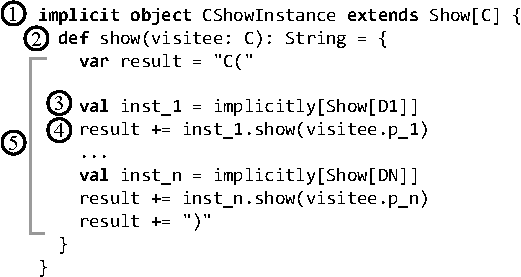
\includegraphics[width=0.87\columnwidth]{basic-generation.pdf}
% \caption{desc.}
% \label{fig:basic-generation}
% \end{figure}

% The basic steps that this algorithm takes are as follows (each numbered step
% corresponds to the numbers shown in the figure):


% % Therefore, we need to define a case
% % class that matches the same shape as both \verb|Fork| and \verb|Leaf|:

% % \begin{math}
% % \texttt{case class}~C(p_1: D_1, \ldots, p_n: D_n)~\{~\bar{m}~\} \\
% % \texttt{~~~~~extends}~E_1~\texttt{with}~ \ldots ~\texttt{with}~E_m
% % \end{math}


% \begin{enumerate}
% \item Definition of an \emph{implicit object} that extends the type of the
%       type class instance (\eg \verb|Show[Tree]|) we'd like to generate. Note here that

% \item
% \end{enumerate}


% % The following is one such example,

% % The pattern assumes that the type class has the
% % following shape:
% % Importantly, for now we only consider type classes with a single type
% % parameter. Moreover, the type class is supposed to have a single (abstract)
% % method that has a single parameter of the generic type and some return type
% % that (a) does not depend on the generic type, and (b) is a monoid.

% % \begin{lstlisting}
% % implicit object CShowInstance extends Show[C] {
% %   def show(visitee: C): String = {
% %     var result = "C("

% %     val inst_1 = implicitly[Show[D1]]
% %     result += inst_1.show(visitee.p_1)
% %     ...
% %     val inst_n = implicitly[Show[DN]]
% %     result += inst_n.show(visitee.p_n)
% %     result += ")"
% %   }
% % }
% % \end{lstlisting}
% % \noindent

% Given a type class, say \verb|Show[T]|, and a datatype, say \verb|Tree|, the
% self-assembly pattern systematically derives a type class instance
% \verb|Show[Tree]|. Applying the pattern requires the following steps:

% \begin{enumerate}

% \item Definition of an \emph{implicit object} that extends the type of the
%       type class instance (\eg \verb|Show[Tree]|) we'd like to generate.

% \item An implementation of the abstract method, within the implicit object,
%       which provides (implicitly looked-up) instances of the type the type class instance is parameterized
%       upon.

% \item Implicit look-up of instances for the components of the type.

% \item Implementation of the type class according to the shape of the type
%       using the component instances.

% \item Introducing the implicit object into the right scope, so that implicit
%       search locates it.

% \end{enumerate}
% \noindent
% In the following we elaborate on each step.

% \paragraph{Case classes} First, we consider a datatype whose declaration has the shape:

% \begin{math}
% \texttt{case class}~C(p_1: D_1, \ldots, p_n: D_n)~\{~\bar{m}~\} \\
% \texttt{~~~~~extends}~E_1~\texttt{with}~ \ldots ~\texttt{with}~E_m
% \end{math}

% The first step is the definition of an implicit object extending
% \verb|Show[C]|:

% \begin{lstlisting}
% implicit object CShowInstance extends Show[C] {
%   def show(visitee: C): String = ...
% }
% \end{lstlisting}
% \noindent
% We derive an implementation of the \verb|show| method by looking up type class
% instances for each of the class parameters $p_i$ of $C$. Since type class
% instances are declared as implicit values in Scala, we can use the following
% method \verb|implicitly| to look up type class instances:

% \begin{lstlisting}
% def implicitly[T](implicit e: T): T = e
% \end{lstlisting}
% \noindent
% Thus, an invocation \verb|implicitly[Show[D_i]]| returns an instance of
% \verb|Show| for type \verb|D_i|.\footnote{The \texttt{implicitly} method is
% defined in the \texttt{Predef} singleton object in Scala's standard library.}

% Using \verb|implicitly| we can implement the type class instance as follows.
% For each class parameter $p_i$ of $C$, we obtain the corresponding type class
% instance (of type \verb|Show[D_i]|), and use it to obtain a result of type
% \verb|String|. Since \verb|String| is a monoid, we can reduce the results
% obtained for all parameters into a single \verb|String|:

% \begin{lstlisting}
% var result: String = ""
% val inst_1 = implicitly[Show[D_1]]
% result = result + inst_1.show(visitee.p_1)
% ...
% val inst_n = implicitly[Show[D_n]]
% result = result + inst_n.show(visitee.p_n)
% \end{lstlisting}
% \noindent
% Making the \verb|CShowInstance| object \verb|implicit| enables support for
% \emph{recursive types:} if one of the types $D_i = C$, then the corresponding
% invocation \verb|implicitly[Show[D_i]]| simply returns \verb|CShowInstance|.

% \paragraph{Traits} The next step is creating instances for (abstract) traits of the following
% shape:
% \begin{math}
% \texttt{sealed trait}~D~\{~\bar{m}~\}
% \end{math}

% Concrete instances of this type have subtypes (dynamically) which are case
% classes (according to our initial simplified view). Therefore, the type class
% instance for $D$ performs a dynamic dispatch to select a specific instance
% based on the runtime classtype of the object that the type class is applied
% to (\verb|visitee|):

% \begin{lstlisting}
% implicit object DShowInstance extends Show[D] {
%   def show(visitee: D): String =
%     visitee match {
%       case null => ...
%       case v1: C1 =>
%         implicitly[Show[C1]].show(v1)
%       ...
%       case vn: Cn =>
%         implicitly[Show[Cn]].show(vn)
%     }
% }
% \end{lstlisting}
% \noindent
% The classtypes \verb|C1|, ..., \verb|Cn| are all subclasses of trait \verb|D|;
% since \verb|D| is sealed, there cannot be other subclasses.



% \subsection{Generation using macros}
% Suppose the goal is to automatically generate type class instances for a type class \verb|Show[T]|.


\subsection{Customization}
\label{sec:customization}

Generation as provided by \selfassembly is convenient, but in some cases it is desirable
to have full control over the type class instances for specific types (one strength of the
type class pattern as introduced in Section~\ref{sec:type-classes}). When using the
\selfassembly library, customization is still possible. It is sufficient to define
custom instances for selected types manually; these custom instances are then transparently
picked up and chosen in place of automatically-generated ones. It is even possible to
use Scala's scoping and implicit precedence rules to prioritize certain instances over
others.

\section{Self-Assembly for Object Orientation}

In this section we talk about all the OO features that we support...

\subsection{Subtyping}

Object-oriented languages like Java or Scala enable the definition of a
\emph{subtyping relation} based on class hierarchies. Given the pervasive use
of subtyping in typical object-oriented programs, our approach is designed to
account for \emph{subtyping polymorphism}. In addition, we provide mechanisms
that enable the object-oriented features even in a setting where
modules/packages are separately compiled.

\subsubsection{Open Hierarchies}

Classes defined in languages like Java are by default ``open,'' which means
that they can have an unbounded number of subclasses spread across several
compilation units. By contrast, \emph{final classes} cannot have subclasses at
all. In addition, \emph{sealed classes} in Scala can only have subclasses
defined within the same compilation unit.

\begin{figure}
\centering
\begin{lstlisting}
// File PersonA.scala:
abstract class Person {
  def name: String
  def age: Int
}
case class Employee(n: String, a: Int, s: Int)
  extends Person {
  def name = n
  def age = a
}

// File PersonB.scala:
case class Firefighter(n: String, a: Int, s: Int)
  extends Person {
  def name = n
  def age = a
  def since = s
}
\end{lstlisting}
  \caption{Open class hierarchy}
  \label{fig:class-hierarchy}
\end{figure}

Our approach enables the generation of type class instances even for open
classes. For example, consider the class hierarchy shown in
Figure~\ref{fig:class-hierarchy}. The \selfassembly library can automatically generate
an instance for type \verb|Person|:

\begin{lstlisting}
val em = Employee("Dave", 35, 80000)
val ff = Firefighter("Jim", 40, 2004)
val inst = implicitly[Show[Person]]
println(inst.show(em))
// prints: Employee(Dave, 35, 80000)
println(inst.show(ff))
// prints: Firefighter(Jim, 40, 2004)
\end{lstlisting}
\noindent
Note that we are using the same \verb|Show| instance to convert both objects
to strings.

\paragraph{Generation}

Concrete instances of a classtype, such as \verb|Person| in
Figure~\ref{fig:class-hierarchy}, in general have subtypes (dynamically). One approach to
account for subtypes is by building the logic for all possible subtypes into
the type class instance for the supertype, like it is shown in
Figure~\ref{fig:trees} in Section~\ref{sec:pretty-printing-complex}.
However, such an approach does not support open class hierarchies, where new subclasses can be
added in additional compilation units.

To support open class hierarchies, the generation of type class instances for
open classes adds a {\em dispatch step}. For a class like \verb|Person| in
Figure~\ref{fig:class-hierarchy}, a dynamic dispatch is generated to select a
specific type class instance based on the runtime classtype of the object that the type
class is applied to (\verb|visitee|):\footnote{Simplified; handling of \texttt{null} values is omitted for simplicity.}

\begin{lstlisting}
implicit object PersonShowInstance
    extends Show[Person] {
  def show(visitee: Person): String =
    visitee match {
      case v1: Employee =>
        implicitly[Show[Employee]].show(v1)
      case v2: Firefighter =>
        implicitly[Show[Firefighter]].show(v2)
    }
}
\end{lstlisting}

% Concrete instances of this type have subtypes (dynamically) which are case
% classes (according to our initial simplified view). Therefore, the type class
% instance for $D$ performs a dynamic dispatch to select a specific instance
% based on the runtime classtype of the object that the type class is applied
% to (\verb|visitee|):

% \begin{lstlisting}
% implicit object DShowInstance extends Show[D] {
%   def show(visitee: D): String =
%     visitee match {
%       case null => ...
%       case v1: C1 =>
%         implicitly[Show[C1]].show(v1)
%       ...
%       case vn: Cn =>
%         implicitly[Show[Cn]].show(vn)
%     }
% }
% \end{lstlisting}
% \noindent
% The classtypes \verb|C1|, ..., \verb|Cn| are all subclasses of trait \verb|D|;
% since \verb|D| is sealed, there cannot be other subclasses.


\subsubsection{Separate Compilation}

To support subtyping polymorphism not only across different compilation units,
but also across separately-compiled modules,\footnote{In the Scala ecosystem
such modules are typically distributed in separate ``JAR files.''}
\selfassembly provides \emph{dynamic instance registries}. In the case of
separately-compiled modules, subclasses for which we would like to generate
instances are in general only discovered at link time. To be able to discover
such subclasses, \selfassembly allows registering generated instances
with an \emph{instance registry} at runtime. A reference to such an
instance registry can then be shared across separately-compiled modules.

For example, module A could create a registry and populate it with a number of
instances:
\begin{lstlisting}
implicit val reg = new SimpleRegistry[Show]
reg.register(classOf[Employee],
             implicitly[Show[Employee]])
reg.register(classOf[Firefighter],
             implicitly[Show[Firefighter]])
...
\end{lstlisting}
\noindent
Note that the registry \verb|reg| is defined as an \emph{implicit value;} as we
explain in the following, this is required to enable registry look-ups when
dispatching to type class instances based on objects' runtime types.

With the instance registry set up in this way, another separately-compiled
module B is then able to dispatch to instances registered by module A:

\begin{lstlisting}
implicit val localReg = getRegistryFrom(moduleA)
localReg.register(classOf[Judge],
                  implicitly[Show[Judge]])
...
\end{lstlisting}
\noindent
Importantly, when module B invokes the \verb|show| method of an instance
\verb|instP| of type \verb|Show[Person]|, passing an object with dynamic type
\verb|Employee|, the generated instance \verb|instP| dispatches to the correct
type class instance of type \verb|Show[Employee]| through a look-up in
registry \verb|localReg|.

\paragraph{Generation mechanics}

To enable registry look-ups, we augment the dispatch logic with a default
case:\footnote{Minimally simplified; the actual code also keeps track of object
identities as discussed further below.}
\begin{lstlisting}
case _ =>
  val registry$1: Registry[Show] =
    implicitly[Registry[Show]]
  val lookup$2: Option[Show[_]] =
    registry$1.get(clazz)
  lookup$2.get
          .asInstanceOf[Show[Person]]
          .show(visitee)
}
\end{lstlisting}


\subsection{Object Identity}

In object-oriented languages like Scala, it is important to take \emph{object
identity} into account. Simple datatypes as shown in
Figure~\ref{fig:type-syntax} already permit cycles in object graphs via re-assignable
fields (using the \verb|var| modifier). It is therefore important to keep
track of objects that have already been visited to avoid infinite recursion.

To enable the detection of cycles in object graphs, we keep track of all
``visited'' objects during the object graph traversal performed by a type
class instance. However, it is not sufficient to maintain a single, global set
of visited objects, since implementations of one type class might depend on
other type classes; different type class instances could therefore interfere
with each other when accessing the same global set (yielding nonsensical
results). Thus, it is preferable to pass this set of visited objects on the
call stack. With the mechanics introduced so far, this is not possible.

To enable passing an additional context (the set of visited objects) on the call stack,
we require type classes to extend \\\verb|Queryable[T, R]|:

\begin{lstlisting}
trait Queryable[T, R] {
  def apply(visitee: T, visited: Set[Any]): R
}
\end{lstlisting}
\noindent
The \verb|Queryable[T, R]| trait declares an \verb|apply| method with an
additional \verb|visited| parameter (compared to the trait of the type class),
which is passed the set of visited objects. This extra method allows us to
distinguish between top-level invocations of type class methods and inner
invocations (of \verb|apply|). The only downside is that custom type class
instances are slightly more verbose to define, although the implementation of
\verb|apply| can typically be a trivial forwarder.

For example, consider the \verb|Show[T]| type class, now extending
\verb|Queryable[T, R]|:
\begin{lstlisting}
trait Show[T] extends Queryable[T, String] {
  def show(visitee: T): String
}
\end{lstlisting}
\noindent
A type class instance for integers can be implemented as follows:
\begin{lstlisting}
implicit val intHasShow = new Show[Int] {
  def show(visitee: Int): String = "" + x
  def apply(visitee: Int, visited: Set[Any]) =
    show(visitee)
}
\end{lstlisting}
\noindent
Note that the implementation of \verb|apply| is trivial.

To enable the detection of cycles in object graphs it is necessary to
adapt the implementation of the implicit object as follows.

\begin{lstlisting}
implicit object CShowInstance extends Show[C] {
  def show(visitee: C): String =
    apply(visitee, Set[Any]())
  def apply(visitee: C, visited: Set[Any]) =
    ...
}
\end{lstlisting}
\noindent
Note that an invocation of \verb|show| is treated as a \emph{top-level
invocation} forwarding to \verb|apply| passing an empty set of visited
objects. Crucially, when applying the type class instances for the class
parameters of $C$, instead of invoking \verb|show| directly, we invoke
\verb|apply| passing the \verb|visited| set extended with the current object
(\verb|visitee|).

\begin{lstlisting}
var result: String = ""
if (!visited(visitee.p_1)) {
  val inst_1 = implicitly[Show[D_1]]
  result = result +
   inst_1.apply(visitee.p_1, visited + visitee)
}
...
if (!visited(visitee.p_n)) {
  val inst_n = implicitly[Show[D_n]]
  result = result +
   inst_n.apply(visitee.p_n, visited + visitee)
}
\end{lstlisting}
\noindent


\section{Queries and Transformations}\label{sec:queries-transformations}

The library provides a set of traits for expressing generic functions that are
either (a) queries or (b) transformations. Basically, a query generates type
class instances that traverse an object graph and return a single result of a
possibly different type. In contrast, a transformation generates type class
instances that perform a deep copy of an object graph, applying
transformations to reachable objects of selected types...


\section{Meta-Programming and Type Classes for Language Extensions}
\label{sec:language-extensions}

In this section we show how our approach supports the definition of {\em
lightweight language extensions} that go beyond object-oriented DGP as
discussed in the previous sections. In particular, the self-assembly pattern
allows defining custom type-based properties that can be type-checked by the
existing Scala type checker.

% An important characteristic of the self-assembly pattern and library is that
% it is a {\em compile-time} generic programming pattern. In addition to having
% access to query and transformation facilities provided by the library, users
% also have access to full type information and Scala's meta-programming API,
% enabling one to generatively define {\em lightweight language extensions}.
% beyond runtime datatype generic programming patterns.

The key to support both object-oriented DGP and lightweight language
extensions is the fact that our approach is based on generic programming {\em
at compile time}. In addition to having access to query and transformation
facilities provided by the library, users also have (a) access to full static
type information and (b) Scala's meta-programming API, enabling one to
generatively define {\em lightweight language extensions}.

The enabled language extensions are lightweight in the sense that they cannot
extend the existing syntax or change Scala’s existing type-checking. Instead,
they can be thought of as pluggable type system
extensions~\cite{PluggableTypes} in that without changing the existing
typechecker, additional properties can be checked. As a result, our approach
supports extensions such as (transitive) type-based immutability checking
which goes beyond even advanced proposals for DGP.


%  . refine existing
% typechecking.


Like before, the patterns we are going to discuss are implemented in our \selfassembly library. Beyond providing re-usable abstractions, our library also serves as a layer between Scala’s macro system and users wishing to define type-system extensions. In this way, the library enforces a principled use of macros\todo{we probably need to qualify this...}, in addition to the typed expression trees discussed in Section~\ref{where we use Expr[String] the first time}.

Section 6.1 introduces our approach using the example of a type-based property for checking deep immutability. Section 6.2 explains the general pattern implemented in \selfassembly.

\subsection{Example}

In the following section we will discuss one such example, a type property for
deep immutability.

Basically, the idea is that macros enable (a) inspecting the full static type
information and (b) generating arbitrary terms (locally). This can be
exploited to derive rich type-based properties such as deep immutability.

For example, deep immutability can be expressed as shown in
Figure~\ref{fig:immutable} (executable code using the \selfassembly library).

\begin{figure}
\centering
\begin{lstlisting}
trait Immutable[T] {
  def noop(x: T): Unit
}

object Immutable extends Property {
  def mkTrees[C <: Context with Singleton](c: C)
    : Trees[C] = new Trees(c)

  class Trees[C <: Context with Singleton]
    (override val c: C) extends super.Trees(c) {
    def check(tpe: c.Type): Unit = {
      import c.universe._
      // if tpe has var, abort
      val allAccessors = tpe.decls.collect {
        case meth: MethodSymbol if meth.isAccessor
          || meth.isParamAccessor => meth }
      val varGetters   = allAccessors.collect {
        case meth if meth.isGetter &&
          meth.accessed != NoSymbol &&
            meth.accessed.asTerm.isVar => meth }
      if (varGetters.nonEmpty) {
        c.abort(c.enclosingPosition,
                "not immutable")
      }
    }
  }

  implicit def generate[T]: Immutable[T] =
    macro genQuery[T, this.type]

  implicit val intIsImmutable =
    new Immutable[Int] { def noop(x: Int) = {} }
  implicit val stringIsImmutable =
    new Immutable[String] { def noop(x: String) = {} }
}
\end{lstlisting}
  \caption{Deep immutability checking using \selfassembly}
  \label{fig:immutable}
\end{figure}

Elements like trait \verb|Property| and the \verb|genQuery| macro are provided by the
library. The idea is that when the \verb|genQuery| macro derives an instance of
\verb|Immutable[T]| it (a) creates an instance of class \verb|Trees| at compile time, and
(b) uses this to check that type $T$ (accessible at compile time as \verb|tpe|) does
not contain vars and it is possible to derive \verb|Immutable| instances for all its
fields (in turn guaranteeing that they are all deeply immutable).

\subsection{Principles}

Oliveira et al.~\cite{Oliveira2010} present the idea of introducing relations
on types using Scala’s implicits.

\subsubsection{Defining unary type relations}

Using implicits a unary type relation can be defined in Scala using a generic
type constructor TC[A]. A type T can de declared to be an element of this
relation, by defining an {\em implicit value} of type TC[T]:

\begin{lstlisting}
implicit val tct = new TC[T] {}
\end{lstlisting}
\noindent

This way, an arbitrary {\em bounded} unary type relation can be defined. The
membership of a type U in the relation TC can be checked by requiring evidence
for it using an implicit parameter:

\begin{lstlisting}
def m[U](implicit ev: TC[U]): ...
\end{lstlisting}
\noindent

(Classes, and thereby constructors, can also have such implicit parameters.)
(Only if there exists an implicit value of type \verb|TC[U]| can an invocation
(of method \verb|m| be type-checked.

Polymorphic implicit methods allow defining a certain class of unbounded type
relations by returning values of type \verb|TC[V]| for multiple types V. For
example, the following implicit method declares all types that are equal to or
subtypes of type Person to be elements of relation \verb|TC|:

\begin{lstlisting}
implicit def belowPerson[S <: Person]: TC[S] = new TC[S] {}
\end{lstlisting}
\noindent

However, without meta-programming the domain of the relation can only be
restricted using type bounds; this is not enough for rich properties such as
immutability. In our approach, it is possible to define relations taking deep
structural type information into account by generating implicit instances
based on the properties of {\em type tags;} user-defined properties inspect
such type tags at compile time. A type tag (which is part of Scala’s meta-
programming API) provides access to the full static type and symbol
information that is otherwise only accessible to the compiler. As a result,
the type relations that our approach and library support are:

\begin{itemize}
\item unbounded (since it’s possible to generate instances for an unbounded number of types), and
\item based on deep structural type information.
\end{itemize}

\section{Implementation}

We provide re-usable building blocks of our approach in the form of a Scala
library.\footnote{See \url{https://github.com/phaller/selfassembly}} The
library has been developed and tested using the current stable release of
Scala, Scala 2.11. No extension of the Scala language or compiler is required
by the library. The library comprises around 2,700 LOC.
% (including whitespace
% and comments).\footnote{We used the following command: \texttt{git ls-files |
% grep scala | xargs wc -l}}

% It should be possible to use the library also with Scala 2.10, since no features
% particular to Scala 2.11 are used...

\paragraph{Use of Macros} As explained in previous sections, our
implementation is based on Scala's macro support~\cite{Burmako2012} which was
introduced in Scala 2.10 as an experimental feature. The Scala release version
2.11 distinguishes between two kinds of macros: \emph{blackbox} and
\emph{whitebox} macros. The essential difference between the two kinds has to
do with type-checking: To determine the type of an invocation of a whitebox
macro, the compiler has to expand the macro first. In contrast, to determine
the type of an invocation of a blackbox macro, no macro expansion is
necessary. As a result, one can reason about the types of blackbox macros (and
their invocations) using just their type signatures (which look just like
method signatures). It is currently unclear, whether whitebox macros will
become a non-experimental feature of a future Scala release.
% \footnote{Personal
% communication with Martin Odersky, Spring 2014.}

Importantly, the implementation of our library requires only blackbox macros.

\subsection{Implemented Examples}

Using \selfassembly, we have implemented the following type classes and
generic functions...

\subsection{Case Study: Scala Serialization}

% Report on examples implemented. Report on port of scala-pickling to \selfassembly and percentage of functionality
% achieved already and how much the code size was reduced and improved in terms of structure.

\section{Related Work}
\label{sec:related-work}

Our work is distinctive from previous work in various ways.  Firstly,
when compared to existing DGP approaches, it supports challenging OO
features such as subtyping or object identity.  Secondly \selfassembly
builds on a type-safe macro mechanism. While there are some DGP approaches
that use macro mechanisms too, these mechnisms tend to be untyped.
Finally our work is more general than DGP in that it also allows the
definition of generic properties like immutability checking.
In what follows we discuss related work in more detail.

\paragraph{DGP in Functional Languages} 
The idea of DGP originated in the Functional Programming community.
Thereare several approaches for writing datatype-generic
programs. Early approaches were based on programming languages with
built-in support for DGP. These approaches include PolyP~\cite{},
Generic Haskell~\cite{}, and Charity~\cite{}. Later approaches were
based on small language extensions added to general purpose languages
like Haskell. Examples include Scrap Your Boilerplate~\cite{} and
Template Haskell~\cite{}.  More recently, researchers have realized
that by using advanced type system features DGP could be implemented
directly as libraries. Extensive surveys of various approaches to DGP
in Haskell (mostly focused on libraries) document various approaches.

\paragraph{DGP in OO Languages}

and
Adaptive Object-Oriented Program- ming [Lieberherr, 1996].

\paragraph{Compile-time Meta-Programming}

\paragraph{Other Related Work}

DGP shares some goals with
reflection and meta-programming techniques. 
Run-time reflection mechanisms (as the one in Java) are
not type-safe (type-errors can occur at run-time), so they cannot be
used as a DGP mechanism. Moreover, some compile-time meta-programming
techniques are untyped: although type-errors are reported at
compile-time they are reported in terms of generated code instead of
the original code.

\cite{TemplateYourBoilerplate}
\cite{Pickling}
\cite{SYB}

% \appendix
% \section{Appendix Title}

% This is the text of the appendix, if you need one.

% \acks

% Acknowledgments, if needed.

% We recommend abbrvnat bibliography style.

\bibliographystyle{abbrvnat}
\bibliography{bib}

% \bibliographystyle{abbrvnat}

% % The bibliography should be embedded for final submission.

% \begin{thebibliography}{}
% \softraggedright

% \bibitem[Smith et~al.(2009)Smith, Jones]{smith02}
% P. Q. Smith, and X. Y. Jones. ...reference text...

% \end{thebibliography}


\end{document}

%                       Revision History
%                       -------- -------
%  Date         Person  Ver.    Change
%  ----         ------  ----    ------

%  2013.06.29   TU      0.1--4  comments on permission/copyright notices

